\chapter{Obesity associated genetic signatures and pathway signatures}
\label{cha:obesity_associated_genetic_signature_and_pathway_signatures}

In this chapter, the underlying biological mechanism of the obesity associated signatures from Creighton's data were investigated.
In doing so, Gatza's pathway genetic signatures were utilised to determine which biological pathways the obesity associated genetic signatures were most similar to.
First, the direction of Gatza's pathway associated genetic signatures were resolved; then the pathway associated metagenes were compared with the obesity associated metagenes; and lastly linear models were constructed based on the pathway metagenes and sample \gls{bmi}/\gls{bmi} status to predict the obesity associated metagenes.

\section{Pathway associated genetic signatures from \citet{Gatza2010a} study}
\label{sec:pathway_associated_genetic_signatures_from_gatza2010a_study}

Pathway associated genetic signatures from the \citet{Gatza2010a} study were examined for their consistency with the reported results.
In the \citet{Gatza2010a} study, their data comprised of samples from different data sets from other studies, \gls{mas}-normalised and the metagene scores were ranked with probit.
However, the analyses so far have used \gls{rma}-normalisation method and ranked based on the number of samples present in the data.
To decide which normalisation or ranking methods were suitable for the analysis, the different methods were compared in Gatza's data (see \cref{app:b}).
Results shown in \cref{app:b} clarified that there was no significant difference in the ranking methods used.
Correlation and scatter plots of the different combinations of transformation matrices (derived from either \gls{rma}- or \gls{mas}-normalised data) with \gls{rma}- or \gls{mas}-normalised data.
It seemed like the normalisation methods of the data in which the transformation matrices were applied to had the most significant effect on the resulting metagenes, rather than the transformation matrices themselves (\cref{app:b}).
This meant that all of the data sets had to be normalised with a single normalisation method, so \gls{rma} normalisation method was used as this method was more reliable than the \gls{mas} method.
Therefore, Gatza's data set was batch corrected first (\cref{sub:batch_correction}), then normalised with \gls{rma} method and the scores were ranked based on the number of samples in the data set.

One thing to be noted from these scatter plots was that there were some pathway signatures that were more variable than the others.
As an example, the \gls{tgfb} metagenes were significantly more dispersed compared to the \gls{pr} metagenes, even though these metagenes were both generated similarly in the same data set (add figure).
These differences were seen in other data sets as well (\cref{app:b}).
This result provided evidence that some of the pathway genetic signatures from the \citet{Gatza2010a} study were more consistent across different data sets than the others.
\\

\noindent
Before Gatza's pathway metagenes were compared with the obesity associated metagenes, the direction of Gatza's pathway metagenes had to be checked to make sure the metagenes were in the correct direction (\cref{sub:metagene_direction}).
% Each pathway metagenes was generated from Gatza's data set and the direction of the metagene was checked with the expression of the representative pathway gene (\cref{tab:metagene_direction}), and the groupings of the pathways were considered as well.
The correlation of all the pathway metagenes with one another were plotted as a heatmap in \cref{fig:gatza_meta_dir}.
The most prominent group had five pathways (E2F1, \gls{pi3k}, Myc, \gls{bcat} and Ras) that clustered at the top right hand corner of the heatmap.
% TODO: add additional info about why these pathways clustered together?
Other groups included \gls{ifna}/\gls{ifny}/\gls{tnfa} pathways, \gls{er}/\gls{pr}/p53 pathway and p63/\gls{her2} pathways.
In addition to these highly correlated groups, \gls{stat3}/\gls{tgfb}/Src/\gls{egfr}/Akt pathways showed little correlation with one another.
Comparing these groups with the results presented by \citet{Gatza2010a} (see \cref{app:b}), the identified groups approximately resembled the groups identified in their study, which confirmed that the directions of Gatza's pathway metagenes were similar to those used in the \citet{Gatza2010a} study.

\begin{figure}[htpb]
	\centering
	\includegraphics[page=15,width=0.7\linewidth]{results2/gatza_meta_trans}
	\caption{Gatza metagene direction}
	\label{fig:gatza_meta_dir}
\end{figure}

To see whether the directionality of Gatza's pathway metagenes were being transferred across to other data sets properly, pathway metagenes were generated in other data sets with the transformation matrices and the groupings of the metagenes were examined.
Creighton's, FM's and Cris' data were \gls{rma}-normalised and transformation matrices of the pathway genetic signatures (derived from Gatza's data set) were applied to the data sets.
The metagenes were plotted in a heatmap (shown in \cref{app:b}), which showed similar groupings  as seen in \cref{fig:gatza_meta_dir}.
This result confirmed that the pathway metagenes were acting similarly in all the data sets in which the transformation matrices have been applied to.

% In order to investigate what the underlying biological mechanism of the obesity associated genetic signatures was, Gatza's pathway associated genetic signatures were used to create linear models to predict the obesity associated metagene scores.
% Before linear models were created, Gatza's pathway metagenes were checked for their directionality to ensure that the pathway metagenes were acting as reported by \citet{Gatza2010a} (see \cref{sub:metagene_direction}).

\section{Pathway associated metagenes and obesity associated metagenes}
\label{sec:pathway_associated_metagenes_and_obesity_associated_metagenes}

Results from previous section confirmed that the pathway metagenes from the \citet{Gatza2010a} study were in the correct directions, and that the pathway metagenes were behaving as expected in different data sets.
Now that the directions of the pathway metagenes were established, these metagenes were ready for comparison with the obesity associated metagenes.
However, all of the pathway metagenes were derived from Gatza's data, whereas the majority of the obesity associated metagenes were derived from Creighton's data, which presents a problem of deciding on which data set the transformation matrices should be generated in.

In theory, the metagenes generated from the application of \gls{svd} and the metagenes generated from transformation matrix would be exactly the same if the transformation matrix was derived from the same data set.
For example, an obesity associated metagene generated from Creighton's data with \gls{svd} would have the same values as the metagenes generated in Creighton's data with the transformation matrix (where the transformation matrix was derived from Creighton's data).
Furthermore, if the \gls{svd}-derived metagenes and transformation matrix-derived metagenes were the same (or at least similar) in a different data set, this suggests that there was no difference in the data sets, at least in terms of the expression of the genetic signatures being investigated.
In other words, the transformation matrix can be made in either the original data set or in a different data set if there was no difference in the \gls{svd}-derived or transformation matrix-derived metagenes.

To decide which data set the transformation matrices for obesity and pathway associated genetic signatures should be generated in, the \gls{svd}- and transformation matrix(TM)-generated metagene scores were compared in all of the data sets.
As in \cref{sec:pathway_associated_genetic_signatures_from_gatza2010a_study}, all data sets were normalised with the \gls{rma} method and metagenes were ranked based on the number of samples in each data set.
Transformation matrices for the obesity associated genetic signatures were made in Creighton's data set and pathway associated genetic signatures were made in Gatza's data set.
Metagenes for all of the obesity and pathway associated genetic signatures were generated in all of the data sets with \gls{svd} and transformation matrices.
The Spearman correlation of the \gls{svd}-generated and TM-generated metagene scores were calculated for each genetic signatures (\cref{tab:svd_vs_tm_path,tab:svd_vs_tm_obs}).

\begin{table}[htpb]
	\centering
	\caption{Spearman correlation of the svd vs tm metagenes (pathway)}
	\label{tab:svd_vs_tm_path}
	\begin{tabular}{lcccc}
		& Gatza & Creighton & Cris & Fuentes-Mattei\\
		\hline
		\rule{0pt}{2.25ex}Akt & 1.000 & 0.5190 & 0.5900 & 0.5563 \\
		\gls{bcat}            & 1.000 & 0.9897 & 0.9977 & 0.9905 \\
		E2F1                  & 1.000 & 0.9646 & 0.8438 & 0.9193 \\
		\gls{egfr}            & 1.000 & 0.0430 & 0.3358 & 0.4040 \\
		\gls{er}              & 1.000 & 0.9978 & 0.9942 & 0.9966 \\
		\gls{her2}            & 1.000 & 0.9553 & 0.5817 & 0.9794 \\
		\gls{ifna}            & 1.000 & 0.9830 & 0.9991 & 0.9951 \\
		\gls{ifny}            & 1.000 & 0.9086 & 0.9950 & 0.9718 \\
		Myc                   & 1.000 & 0.9878 & 0.9852 & 0.9689 \\
		p53                   & 1.000 & 0.3808 & 0.9981 & 0.7923 \\
		p63                   & 1.000 & 0.8319 & 0.2951 & 0.8368 \\
		\gls{pi3k}            & 1.000 & 0.9543 & 0.5989 & 0.9365 \\
		\gls{pr}              & 1.000 & 0.9511 & 0.9887 & 0.9845 \\
		Ras                   & 1.000 & 0.9078 & 0.9125 & 0.7229 \\
		Src                   & 1.000 & 0.9575 & 0.7173 & 0.9548 \\
		\gls{stat3}           & 1.000 & 0.1902 & 0.9159 & 0.6167 \\
		\gls{tgfb}            & 1.000 & 0.9918 & 0.2543 & 0.9890 \\
		\gls{tnfa}            & 1.000 & 0.6046 & 0.9365 & 0.4315 \\

	\end{tabular}
\end{table}

\begin{table}[htpb]
	\centering
	\caption{Spearman correlation of the svd vs tm metagenes (obesity)}
	\label{tab:svd_vs_tm_obs}
	\begin{tabular}{lcccc}
		& Creighton & Gatza  & Fuentes-Mattei & Cris\\
		\hline
		\rule{0pt}{2.25ex} Cr & 1.000     & 0.9985 & 0.9872 & 0.9161 \\
		Res                   & 1.000     & 0.9987 & 0.9898 & 0.9652 \\
		CrOl                  & 1.000     & 0.9982 & 0.9926 & 0.9715 \\
		ResOl                 & 1.000     & 0.9981 & 0.9927 & 0.9571 \\
		Ca                    & 1.000     & 0.9985 & 0.9893 & 0.9468 \\
		CaRes                 & 1.000     & 0.9988 & 0.9939 & 0.9865 \\
		CaOl                  & 1.000     & 0.9983 & 0.9937 & 0.9677 \\
		CaResOl               & 1.000     & 0.9984 & 0.9952 & 0.9642 \\
		Original              & 1.000     & 0.9928 & 0.9862 & 0.9344 \\
	\end{tabular}
\end{table}

In \cref{tab:svd_vs_tm_path,tab:svd_vs_tm_obs}, the obesity and pathway associated genetic signatures had a correlatin of 1 in Creighton's and Gatza's data sets respectively, as the transformation matrices were generated in those data sets.
The correlations of the obesity and pathway metagenes were variable across different data sets, which was as expected since all the data sets were different from one another.
However, what was unexpected was the fact that there were some genetic signatures that were highly correlated in all of the data sets, whereas the metagene correlation of other signatures were highly variable across different data sets.
For example, the \gls{bcat} pathway metagene was highly correlated in all of the data sets (\textgreater{} 0.98), whereas the \gls{stat3} pathway metagene was variable across different data sets, ranging from 0.1902 to 0.9159 (\cref{tab:svd_vs_tm_path,fig:allmetacor_bar}).
The fact that some pathway associated metagenes were consistent across different data sets suggested that some of these genetic signatures were reliable and did not depend on the data set the transformation matrices were derived from.
On the other hand, the genetic signatures that were not consistent across the data sets were likely to be dependent on the data set in which they were derived from, and therefore the transformation matrices for these signatures must be derived from Gatza's data set.

In contrast to the pathway associated genetic signatures, all of the obesity associated genetic signatures showed high correlation of the \gls{svd}- and transformation matrix-generated metagenes across the different data sets.
This suggested that obesity associated genetic signatures were consistent across all data sets and the transformation matrices for these signatures could be made in any of the data sets.
Taken together, transformation matrices for all the genetic  signatures were decided to be made in the Gatza's data set, since there were some pathway associated signatures that were specific to Gatza's data, but none of the obesity associated genetic signatures were specific to a data set.
\\

\begin{figure}[htpb]
	\centering
	\includegraphics[page=2,width=0.45\linewidth]{results2/allmetacor_bar}
	\includegraphics[page=16,width=0.45\linewidth]{results2/allmetacor_bar}
	\caption{Visual comparison of the correlation of the metagenes across different data sets}
	\label{fig:allmetacor_bar}
\end{figure}

\noindent
To visually determine which pathway associated genetic signatures were most similar to the obesity associated genetic signatures, heatmaps were created with the metagenes for all of the genetic signatures.
The directions of the pathway associated metagenes have already been determined in \cref{sec:pathway_associated_genetic_signatures_from_gatza2010a_study}, and the directions of the obesity associated metagenes were checked in Gatza's data set as described in \cref{sub:metagene_direction}.
All of the metagenes were created in \gls{rma}-normalised Gatza's data set with \gls{svd}, and the metagene scores were plotted in a heatmap and clustered into groups (\cref{fig:gatza_allmeta}).

\begin{figure}[htpb]
	\centering
	\includegraphics[page=15,width=0.8\linewidth]{results2/all_meta_trans}
	\caption{All metagenes in Gatza's data}
	\label{fig:gatza_allmeta}
\end{figure}

From \cref{fig:gatza_allmeta}, all of the obesity associated metagenes from Creighton's data set clustered together into a group, but none of the pathway associated metagenes associated strongly with the obesity metagenes.
Though \gls{her2} and p63 pathway metagenes were grouped next to the cluster of obesity metagenes, the similarity was at most about 0.6.
Fuentes-Mattei's obesity associated metagene did not cluster together with the obesity metagenes from Creighton's data set, nor with any of the other pathway metagenes.
The fact that Fuentes-Mattei's metagene did not cluster with Creighton's metagenes showed that the nature of Fuentes-Mattei's metagene was different from those metagenes found in Creighton's data set.
Furthermore, their metagene did not cluster with Gatza's Akt pathway in the heatmap, even though \citet{Fuentes-Mattei2014} provided clear evidence that their metagene specifically activated the Akt/\gls{mtor} signalling pathway in a mouse model.
This may have been due to the lack of consistency of the Akt pathway signature in different data sets (\cref{tab:svd_vs_tm_path}).
Another likely reason could be that Fuentes-Mattei's genetic signature was not comprised only of the genes from the Akt pathway, but genes from other pathways as well, and so the metagene did not cluster together with the Akt pathway signature in the heatmap.

The results in this section suggested that none of the obesity associated genetic signatures were similar or related to any of the pathway associated genetic signatures from the \citet{Gatza2010a} study.

(add heatmaps of other data (Creighton/FM/Cris) as well? or maybe in appendix)

\section{Prediction of obesity associated metagene with pathway associate metagene}
\label{sec:prediction_of_obesity_associated_metagene_with_pathway_associate_metagene}

% and lastly linear models were constructed based on the pathway metagenes and sample \gls{bmi}/\gls{bmi} status to predict the obesity associated metagenes.

To confirm that the obesity associated metagenes were not related to any of the biological pathway signatures from the \citet{Gatza2010a} study, linear models were created to predict the obesity metagene scores with the pathway metagene scores.
If any of the pathway metagenes were significant in the linear model, this provided evidence that the significant pathways in the linear model were related to the obesity metagene.
Since most of the obesity metagenes were found in Creighton's data set and only Creighton's and Cris' data sets had \gls{bmi}/\gls{bmi} status information for the samples, Cris' data set was used as the training data set to create linear models for obesity metagene score prediction.

Metagene scores used for the construction of linear models were generated from the application of the transformation matrices derived from Gatza's data (from \cref{sec:pathway_associated_metagenes_and_obesity_associated_metagenes}) to \gls{rma}-normalised Cris' data.
For each of the obesity metagenes identified, seven linear models were created: \gls{bmi}-only, \gls{bmi} status-only, \gls{bmi} and \gls{bmi} status, pathway metagenes-only, and all of the combinations of pathway metagenes with \gls{bmi} and/or \gls{bmi} status.

\begin{table}[htpb]
	\centering
	\caption{caption}
	\label{tab:lm_sig_var}
	\begin{tabular}{llcc}
		Linear Model & Variables & Estimate & P-value\\
		\hline
		\gls{\gls{bmi}}-only                                 & \gls{bmi}  & -0.001481 & 0.717      \\
		\gls{\gls{bmi}} status-only                          & Obese      & -0.09809  & 0.166      \\
                                                             & Overweight & -0.01263  & 0.871      \\
		\gls{\gls{bmi}} and \gls{\gls{bmi}} status           & \gls{bmi}  & 0.01087   & 0.1232     \\
                                                             & Obese      & -0.24812  & 0.0398 *   \\
                                                             & Overweight & -0.06873  & 0.4199     \\
		Pathways only                                        & \gls{bcat} & 0.091552  & 0.6765     \\
                                                             & \gls{er}   & 0.052266  & 0.8342     \\
                                                             & \gls{ifna} & -0.499303 & 0.3070     \\
                                                             & \gls{ifny} & 0.422406  & 0.3983     \\
                                                             & myc        & -0.003752 & 0.9867     \\
                                                             & \gls{pr}   & 0.583569  & 0.0164   * \\
		\gls{\gls{bmi}} and Pathways                         & \gls{bmi}  & -0.002368 & 0.5271     \\
                                                             & \gls{bcat} & 0.112118  & 0.6144     \\
                                                             & \gls{er}   & 0.054001  & 0.8294     \\
                                                             & \gls{ifna} & -0.538290 & 0.2763     \\
                                                             & \gls{ifny} & 0.466144  & 0.3576     \\
                                                             & myc        & 0.016832  & 0.9411     \\
                                                             & \gls{pr}   & 0.592696  & 0.0154   * \\
		\gls{\gls{bmi}} and Pathways                         & Obese      & -0.10346  & 0.1125     \\
                                                             & Overweight & -0.01200  & 0.8641     \\
                                                             & \gls{bcat} & 0.14950   & 0.5008     \\
                                                             & \gls{er}   & 0.03263   & 0.8955     \\
                                                             & \gls{ifna} & -0.67067  & 0.1767     \\
                                                             & \gls{ifny} & 0.58879   & 0.2453     \\
                                                             & myc        & 0.04388   & 0.8457     \\
                                                             & \gls{pr}   & 0.57993   & 0.0164   * \\
		\gls{\gls{bmi}}, \gls{\gls{bmi}} status and pathways & \gls{bmi}  & 0.009057  & 0.1614     \\
                                                             & Obese      & -0.229223 & 0.0397   * \\
                                                             & Overweight & -0.057586 & 0.4546     \\
                                                             & \gls{bcat} & 0.145953  & 0.5087     \\
                                                             & \gls{er}   & 0.009057  & 0.9708     \\
                                                             & \gls{ifna} & -0.693675 & 0.1605     \\
                                                             & \gls{ifny} & 0.588958  & 0.2426     \\
                                                             & myc        & 0.026253  & 0.9070     \\
                                                             & \gls{pr}   & 0.544864  & 0.0240   * \\

	
	\end{tabular}
\end{table}

% [1] "rawobsgene"

% Call:
% lm(formula = as.formula(formula_txt[j]), data = data)

% Coefficients:
%              Estimate Pr(>|t|)
% [1] "crolgene"

% Call:
% lm(formula = as.formula(formula_txt[j]), data = data)

% Coefficients:
%              Estimate Std. Error t value Pr(>|t|)
% (Intercept)         0.553214  0.123891 4.465  2.16e-05 ***
% bmi                 -0.001629 0.004071 -0.400 0.69
% (Intercept)         0.55700   0.05464  10.194 <2e-16   ***
% bmiStatusobese      -0.10551  0.07021  -1.503 0.136
% bmiStatusoverweight -0.02165  0.07727  -0.280 0.780
% (Intercept)         0.307513  0.163530 1.880  0.0631   .
% bmi                 0.011279  0.006976 1.617  0.1092
% bmiStatusobese      -0.261145 0.118795 -2.198 0.0304   *
% bmiStatusoverweight -0.079845 0.084661 -0.943 0.3480
% (Intercept)         0.007141  0.382725 0.019  0.9852
% bcat_probes         0.156062  0.223779 0.697  0.4873
% er_probes           0.123403  0.254800 0.484  0.6293
% ifna_probes         -0.430229 0.497301 -0.865 0.3892
% ifng_probes         0.378437  0.509352 0.743  0.4594
% myc_probes          0.160785  0.229142 0.702  0.4846
% pr_probes           0.597403  0.244252 2.446  0.0164   *
% (Intercept)         0.055088  0.389472 0.141  0.8878
% bmi                 -0.002745 0.003814 -0.720 0.4736
% bcat_probes         0.179900  0.226799 0.793  0.4297
% er_probes           0.125413  0.255485 0.491  0.6247
% ifna_probes         -0.475417 0.502546 -0.946 0.3466
% ifng_probes         0.429131  0.515526 0.832  0.4074
% myc_probes          0.184642  0.232124 0.795  0.4284
% pr_probes           0.607982  0.245336 2.478  0.0151   *
% (Intercept)         0.01666   0.37989  0.044  0.9651
% bmiStatusobese      -0.11197  0.06602  -1.696 0.0933   .
% bmiStatusoverweight -0.02348  0.07151  -0.328 0.7434
% bcat_probes         0.22035   0.22616  0.974  0.3325
% er_probes           0.10450   0.25330  0.413  0.6809
% ifna_probes         -0.60343  0.50372  -1.198 0.2341
% ifng_probes         0.54671   0.51484  1.062  0.2911
% myc_probes          0.21341   0.22998  0.928  0.3559
% pr_probes           0.59491   0.24257  2.453  0.0161   *
% (Intercept)         -0.128149 0.393204 -0.326 0.7453
% bmi                 0.008834  0.006565 1.346  0.1819
% bmiStatusobese      -0.234634 0.112386 -2.088 0.0397   *
% bmiStatusoverweight -0.067942 0.078484 -0.866 0.3890
% bcat_probes         0.216892  0.225167 0.963  0.3380
% er_probes           0.081506  0.252745 0.322  0.7478
% ifna_probes         -0.625864 0.501740 -1.247 0.2155
% ifng_probes         0.546873  0.512538 1.067  0.2889
% myc_probes          0.196215  0.229305 0.856  0.3945
% pr_probes           0.560706  0.242816 2.309  0.0232   *

% [1] "resobsgene"

% Call:
% lm(formula = as.formula(formula_txt[j]), data = data)

% Coefficients:
%              Estimate Std. Error t value Pr(>|t|)
% (Intercept)         0.547104  0.123915 4.415  2.62e-05 ***
% bmi                 -0.001422 0.004072 -0.349 0.728
% (Intercept)         0.547619  0.054641 10.022 <2e-16   ***
% bmiStatusobese      -0.096832 0.070212 -1.379 0.171
% bmiStatusoverweight -0.001804 0.077273 -0.023 0.981
% (Intercept)         0.298589  0.163546 1.826  0.0710   .
% bmi                 0.011259  0.006976 1.614  0.1099
% bmiStatusobese      -0.252186 0.118807 -2.123 0.0364   *
% bmiStatusoverweight -0.059898 0.084669 -0.707 0.4810
% (Intercept)         0.18694   0.36963  0.506  0.6142
% bcat_probes         0.09717   0.21612  0.450  0.6541
% er_probes           0.07879   0.24608  0.320  0.7496
% ifna_probes         -0.17576  0.48029  -0.366 0.7152
% ifng_probes         0.07930   0.49193  0.161  0.8723
% myc_probes          -0.04517  0.22130  -0.204 0.8387
% pr_probes           0.59554   0.23590  2.525  0.0133   *
% (Intercept)         0.221757  0.376612 0.589  0.5574
% bmi                 -0.001994 0.003688 -0.540 0.5902
% bcat_probes         0.114479  0.219311 0.522  0.6029
% er_probes           0.080247  0.247050 0.325  0.7461
% ifna_probes         -0.208580 0.485954 -0.429 0.6688
% ifng_probes         0.116119  0.498505 0.233  0.8163
% myc_probes          -0.027845 0.224460 -0.124 0.9015
% pr_probes           0.603222  0.237235 2.543  0.0127   *
% (Intercept)         0.195965  0.367384 0.533  0.5951
% bmiStatusobese      -0.096834 0.063844 -1.517 0.1328
% bmiStatusoverweight -0.004412 0.069155 -0.064 0.9493
% bcat_probes         0.150379  0.218719 0.688  0.4935
% er_probes           0.058880  0.244961 0.240  0.8106
% ifna_probes         -0.344126 0.487134 -0.706 0.4817
% ifng_probes         0.242697  0.497893 0.487  0.6271
% myc_probes          -0.001285 0.222407 -0.006 0.9954
% pr_probes           0.591191  0.234582 2.520  0.0135   *
% (Intercept)         0.041459  0.379420 0.109  0.9132
% bmi                 0.009426  0.006335 1.488  0.1403
% bmiStatusobese      -0.227717 0.108446 -2.100 0.0386   *
% bmiStatusoverweight -0.051853 0.075733 -0.685 0.4953
% bcat_probes         0.146687  0.217273 0.675  0.5013
% er_probes           0.034350  0.243884 0.141  0.8883
% ifna_probes         -0.368065 0.484150 -0.760 0.4491
% ifng_probes         0.242870  0.494570 0.491  0.6246
% myc_probes          -0.019634 0.221267 -0.089 0.9295
% pr_probes           0.554701  0.234304 2.367  0.0201   *

% [1] "rescrolgene"

% Call:
% lm(formula = as.formula(formula_txt[j]), data = data)

% Coefficients:
%               Estimate Std. Error t value Pr(>|t|)
% (Intercept)         0.5343899  0.1239554 4.311  3.9e-05 ***
% bmi                 -0.0009922 0.0040730 -0.244 0.808
% (Intercept)         0.54870    0.05482   10.009 <2e-16  ***
% bmiStatusobese      -0.09063   0.07044   -1.287 0.201
% bmiStatusoverweight -0.01515   0.07753   -0.195 0.845
% (Intercept)         0.304200   0.164179  1.853  0.0670  .
% bmi                 0.011054   0.007003  1.578  0.1178
% bmiStatusobese      -0.243160  0.119267  -2.039 0.0442  *
% bmiStatusoverweight -0.072189  0.084997  -0.849 0.3978
% (Intercept)         0.17069    0.37929   0.450  0.6537
% bcat_probes         0.09532    0.22177   0.430  0.6683
% er_probes           0.03171    0.25251   0.126  0.9004
% ifna_probes         -0.57965   0.49283   -1.176 0.2426
% ifng_probes         0.50919    0.50478   1.009  0.3157
% myc_probes          0.06345    0.22708   0.279  0.7805
% pr_probes           0.54200    0.24206   2.239  0.0276  *
% (Intercept)         0.204758   0.386507  0.530  0.5976
% bmi                 -0.001950  0.003785  -0.515 0.6076
% bcat_probes         0.112257   0.225072  0.499  0.6192
% er_probes           0.033134   0.253540  0.131  0.8963
% ifna_probes         -0.611750  0.498720  -1.227 0.2231
% ifng_probes         0.545210   0.511601  1.066  0.2894
% myc_probes          0.080405   0.230357  0.349  0.7279
% pr_probes           0.549516   0.243468  2.257  0.0264  *
% (Intercept)         0.17933    0.37777   0.475  0.636
% bmiStatusobese      -0.09681   0.06565   -1.475 0.144
% bmiStatusoverweight -0.01219   0.07111   -0.171 0.864
% bcat_probes         0.14969    0.22490   0.666  0.507
% er_probes           0.01354    0.25189   0.054  0.957
% ifna_probes         -0.73888   0.50091   -1.475 0.144
% ifng_probes         0.66381    0.51197   1.297  0.198
% myc_probes          0.10813    0.22869   0.473  0.638
% pr_probes           0.53872    0.24121   2.233  0.028   *
% (Intercept)         0.027729   0.390580  0.071  0.9436
% bmi                 0.009248   0.006522  1.418  0.1596
% bmiStatusobese      -0.225233  0.111636  -2.018 0.0466  *
% bmiStatusoverweight -0.058734  0.077961  -0.753 0.4532
% bcat_probes         0.146066   0.223664  0.653  0.5154
% er_probes           -0.010526  0.251058  -0.042 0.9667
% ifna_probes         -0.762373  0.498391  -1.530 0.1296
% ifng_probes         0.663981   0.509117  1.304  0.1955
% myc_probes          0.090122   0.227775  0.396  0.6933
% pr_probes           0.502919   0.241196  2.085  0.0399  *

% [1] "caobsgene"

% Call:
% lm(formula = as.formula(formula_txt[j]), data = data)

% Coefficients:
%              Estimate Std. Error t value Pr(>|t|)
% (Intercept)         0.538968  0.123943 4.349  3.39e-05 ***
% bmi                 -0.001147 0.004073 -0.282 0.779
% (Intercept)         0.53896   0.05458  9.875  2.76e-16 ***
% bmiStatusobese      -0.08982  0.07013  -1.281 0.203
% bmiStatusoverweight 0.01804   0.07719  0.234  0.816
% (Intercept)         0.27986   0.16317  1.715  0.0896   .
% bmi                 0.01171   0.00696  1.683  0.0957   .
% bmiStatusobese      -0.25146  0.11853  -2.121 0.0365   *
% bmiStatusoverweight -0.04241  0.08447  -0.502 0.6168
% (Intercept)         0.12454   0.38803  0.321  0.7490
% bcat_probes         0.14068   0.22688  0.620  0.5367
% er_probes           0.11597   0.25833  0.449  0.6545
% ifna_probes         -0.33319  0.50420  -0.661 0.5104
% ifng_probes         0.30871   0.51641  0.598  0.5515
% myc_probes          -0.04569  0.23232  -0.197 0.8445
% pr_probes           0.56692   0.24764  2.289  0.0243   *
% (Intercept)         0.162063  0.395326 0.410  0.6828
% bmi                 -0.002148 0.003872 -0.555 0.5804
% bcat_probes         0.159335  0.230208 0.692  0.4906
% er_probes           0.117547  0.259326 0.453  0.6514
% ifna_probes         -0.368552 0.510101 -0.723 0.4718
% ifng_probes         0.348376  0.523276 0.666  0.5072
% myc_probes          -0.027017 0.235613 -0.115 0.9090
% pr_probes           0.575201  0.249024 2.310  0.0232   *
% (Intercept)         0.134514  0.384960 0.349  0.7276
% bmiStatusobese      -0.099695 0.066899 -1.490 0.1397
% bmiStatusoverweight 0.008987  0.072463 0.124  0.9016
% bcat_probes         0.193430  0.229183 0.844  0.4009
% er_probes           0.092451  0.256681 0.360  0.7196
% ifna_probes         -0.522336 0.510440 -1.023 0.3089
% ifng_probes         0.492130  0.521713 0.943  0.3481
% myc_probes          -0.001892 0.233048 -0.008 0.9935
% pr_probes           0.560583  0.245805 2.281  0.0249   *
% (Intercept)         -0.028482 0.397505 -0.072 0.9430
% bmi                 0.009944  0.006637 1.498  0.1376
% bmiStatusobese      -0.237770 0.113616 -2.093 0.0392   *
% bmiStatusoverweight -0.041061 0.079343 -0.518 0.6061
% bcat_probes         0.189535  0.227630 0.833  0.4073
% er_probes           0.066573  0.255509 0.261  0.7950
% ifna_probes         -0.547591 0.507227 -1.080 0.2832
% ifng_probes         0.492312  0.518143 0.950  0.3446
% myc_probes          -0.021250 0.231813 -0.092 0.9272
% pr_probes           0.522087  0.245472 2.127  0.0362   *

% [1] "cacrolgene"

% Call:
% lm(formula = as.formula(formula_txt[j]), data = data)

% Coefficients:
%               Estimate Std. Error t value Pr(>|t|)
% (Intercept)         5.062e-01  1.240e-01 4.083  9.16e-05 ***
% bmi                 -3.953e-05 4.074e-03 -0.010 0.992
% (Intercept)         0.52453    0.05485   9.564  1.29e-15 ***
% bmiStatusobese      -0.06411   0.07047   -0.910 0.365
% bmiStatusoverweight 0.02958    0.07756   0.381  0.704
% (Intercept)         0.273274   0.164135  1.665  0.0992   .
% bmi                 0.011360   0.007001  1.622  0.1080
% bmiStatusobese      -0.220856  0.119235  -1.852 0.0671   .
% bmiStatusoverweight -0.029032  0.084974  -0.342 0.7334
% (Intercept)         0.02932    0.40048   0.073  0.9418
% bcat_probes         0.23660    0.23416   1.010  0.3150
% er_probes           0.09521    0.26662   0.357  0.7218
% ifna_probes         -0.49129   0.52037   -0.944 0.3476
% ifng_probes         0.44466    0.53298   0.834  0.4063
% myc_probes          0.16111    0.23977   0.672  0.5033
% pr_probes           0.49566    0.25558   1.939  0.0555   .
% (Intercept)         0.051698   0.408467  0.127  0.8996
% bmi                 -0.001281  0.004000  -0.320 0.7495
% bcat_probes         0.247720   0.237861  1.041  0.3004
% er_probes           0.096149   0.267946  0.359  0.7205
% ifna_probes         -0.512383  0.527057  -0.972 0.3335
% ifng_probes         0.468320   0.540670  0.866  0.3887
% myc_probes          0.172240   0.243445  0.708  0.4811
% pr_probes           0.500601   0.257301  1.946  0.0548   .
% (Intercept)         0.03806    0.39931   0.095  0.9243
% bmiStatusobese      -0.07973   0.06939   -1.149 0.2536
% bmiStatusoverweight 0.02249    0.07516   0.299  0.7655
% bcat_probes         0.27648    0.23772   1.163  0.2479
% er_probes           0.07298    0.26625   0.274  0.7846
% ifna_probes         -0.66043   0.52946   -1.247 0.2155
% ifng_probes         0.60854    0.54116   1.125  0.2638
% myc_probes          0.19456    0.24173   0.805  0.4230
% pr_probes           0.48849    0.25497   1.916  0.0586   .
% (Intercept)         -0.123986  0.412743  -0.300 0.7646
% bmi                 0.009886   0.006892  1.434  0.1549
% bmiStatusobese      -0.216997  0.117971  -1.839 0.0692   .
% bmiStatusoverweight -0.027267  0.082384  -0.331 0.7414
% bcat_probes         0.272606   0.236356  1.153  0.2518
% er_probes           0.047249   0.265304  0.178  0.8591
% ifna_probes         -0.685542  0.526672  -1.302 0.1964
% ifng_probes         0.608724   0.538006  1.131  0.2609
% myc_probes          0.175314   0.240700  0.728  0.4683
% pr_probes           0.450215   0.254882  1.766  0.0808   .

% [1] "caresobsgene"

% Call:
% lm(formula = as.formula(formula_txt[j]), data = data)

% Coefficients:
%             Estimate Std. Error t value Pr(>|t|)
% (Intercept)         0.462424  0.123913 3.732  0.00032  ***
% bmi                 0.001442  0.004072 0.354  0.72408
% (Intercept)         0.46970   0.05452  8.616  1.39e-13 ***
% bmiStatusobese      0.09338   0.07005  1.333  0.186
% bmiStatusoverweight -0.01840  0.07710  -0.239 0.812
% (Intercept)         0.722057  0.163100 4.427  2.55e-05 ***
% bmi                 -0.011409 0.006957 -1.640 0.1043
% bmiStatusobese      0.250806  0.118483 2.117  0.0369   *
% bmiStatusoverweight 0.040473  0.084438 0.479  0.6328
% (Intercept)         1.1017    0.3815   2.888  0.00483  **
% bcat_probes         -0.2217   0.2230   -0.994 0.32284
% er_probes           -0.2308   0.2540   -0.909 0.36579
% ifna_probes         0.1853    0.4957   0.374  0.70938
% ifng_probes         -0.1528   0.5077   -0.301 0.76408
% myc_probes          -0.0737   0.2284   -0.323 0.74765
% pr_probes           -0.6876   0.2434   -2.825 0.00581  **
% (Intercept)         1.056654  0.388317 2.721  0.00780  **
% bmi                 0.002580  0.003803 0.678  0.49929
% bcat_probes         -0.244104 0.226127 -1.079 0.28322
% er_probes           -0.232713 0.254728 -0.914 0.36335
% ifna_probes         0.227770  0.501056 0.455  0.65049
% ifng_probes         -0.200460 0.513998 -0.390 0.69745
% myc_probes          -0.096122 0.231435 -0.415 0.67888
% pr_probes           -0.697585 0.244608 -2.852 0.00538  **
% (Intercept)         1.09174   0.37821  2.887  0.00488  **
% bmiStatusobese      0.10153   0.06573  1.545  0.12592
% bmiStatusoverweight -0.00544  0.07119  -0.076 0.93926
% bcat_probes         -0.27598  0.22517  -1.226 0.22351
% er_probes           -0.20770  0.25218  -0.824 0.41234
% ifna_probes         0.37360   0.50149  0.745  0.45823
% ifng_probes         -0.33545  0.51257  -0.654 0.51449
% myc_probes          -0.11868  0.22896  -0.518 0.60548
% pr_probes           -0.68170  0.24150  -2.823 0.00586  **
% (Intercept)         1.235747  0.391476 3.157  0.00218  **
% bmi                 -0.008785 0.006537 -1.344 0.18237
% bmiStatusobese      0.223518  0.111892 1.998  0.04881  *
% bmiStatusoverweight 0.038776  0.078139 0.496  0.62094
% bcat_probes         -0.272540 0.224177 -1.216 0.22730
% er_probes           -0.184837 0.251634 -0.735 0.46455
% ifna_probes         0.395907  0.499535 0.793  0.43015
% ifng_probes         -0.335611 0.510285 -0.658 0.51243
% myc_probes          -0.101582 0.228298 -0.445 0.65743
% pr_probes           -0.647688 0.241749 -2.679 0.00879  **

% [1] "carescrolgene"

% Call:
% lm(formula = as.formula(formula_txt[j]), data = data)

% Coefficients:
%              Estimate Std. Error t value Pr(>|t|)
% (Intercept)         0.4928357 0.1239867 3.975  0.000136 ***
% bmi                 0.0004131 0.0040740 0.101  0.919450
% (Intercept)         0.52814   0.05483   9.633  9.13e-16 ***
% bmiStatusobese      -0.06913  0.07045   -0.981 0.329
% bmiStatusoverweight 0.02453   0.07753   0.316  0.752
% (Intercept)         0.232845  0.163204  1.427  0.1569
% bmi                 0.013351  0.006962  1.918  0.0582   .
% bmiStatusobese      -0.253344 0.118558  -2.137 0.0352   *
% bmiStatusoverweight -0.044356 0.084492  -0.525 0.6008
% (Intercept)         -0.1205   0.3891    -0.310 0.7576
% bcat_probes         0.2439    0.2275    1.072  0.2864
% er_probes           0.1383    0.2590    0.534  0.5948
% ifna_probes         -0.4364   0.5056    -0.863 0.3903
% ifng_probes         0.4301    0.5178    0.831  0.4084
% myc_probes          0.2837    0.2330    1.218  0.2264
% pr_probes           0.5789    0.2483    2.331  0.0219   *
% (Intercept)         -0.102321 0.396926  -0.258 0.7972
% bmi                 -0.001038 0.003887  -0.267 0.7900
% bcat_probes         0.252943  0.231140  1.094  0.2767
% er_probes           0.139029  0.260375  0.534  0.5947
% ifna_probes         -0.453502 0.512164  -0.885 0.3782
% ifng_probes         0.449266  0.525393  0.855  0.3947
% myc_probes          0.292758  0.236566  1.238  0.2191
% pr_probes           0.582903  0.250031  2.331  0.0219   *
% (Intercept)         -0.11188  0.38790   -0.288 0.7737
% bmiStatusobese      -0.08019  0.06741   -1.190 0.2373
% bmiStatusoverweight 0.01833   0.07302   0.251  0.8024
% bcat_probes         0.28469   0.23093   1.233  0.2209
% er_probes           0.11686   0.25864   0.452  0.6525
% ifna_probes         -0.60153  0.51434   -1.170 0.2453
% ifng_probes         0.59011   0.52570   1.123  0.2646
% myc_probes          0.31782   0.23483   1.353  0.1793
% pr_probes           0.57227   0.24768   2.311  0.0231   *
% (Intercept)         -0.284628 0.400004  -0.712 0.4786
% bmi                 0.010538  0.006679  1.578  0.1181
% bmiStatusobese      -0.226528 0.114330  -1.981 0.0506   .
% bmiStatusoverweight -0.034711 0.079842  -0.435 0.6648
% bcat_probes         0.280559  0.229061  1.225  0.2239
% er_probes           0.089437  0.257116  0.348  0.7288
% ifna_probes         -0.628292 0.510417  -1.231 0.2216
% ifng_probes         0.590302  0.521401  1.132  0.2606
% myc_probes          0.297308  0.233271  1.275  0.2058
% pr_probes           0.531475  0.247015  2.152  0.0341   *

% [1] "crobsgenes"

% Call:
% lm(formula = as.formula(formula_txt[j]), data = data)

% Coefficients:
%             Estimate Std. Error t value Pr(>|t|)
% (Intercept)         0.456126  0.123888 3.682  0.000381 ***
% bmi                 0.001654  0.004071 0.406  0.685322
% (Intercept)         0.459596  0.054606 8.417  3.7e-13  ***
% bmiStatusobese      0.100893  0.070167 1.438  0.154
% bmiStatusoverweight 0.005772  0.077224 0.075  0.941
% (Intercept)         0.704210  0.163518 4.307  4.04e-05 ***
% bmi                 -0.011059 0.006975 -1.586 0.1162
% bmiStatusobese      0.253491  0.118786 2.134  0.0354   *
% bmiStatusoverweight 0.062836  0.084654 0.742  0.4598
% (Intercept)         1.0667    0.3806   2.803  0.00618  **
% bcat_probes         -0.2284   0.2225   -1.026 0.30740
% er_probes           -0.1481   0.2534   -0.584 0.56041
% ifna_probes         0.4504    0.4945   0.911  0.36477
% ifng_probes         -0.4013   0.5065   -0.792 0.43018
% myc_probes          -0.1402   0.2279   -0.615 0.53986
% pr_probes           -0.6446   0.2429   -2.654 0.00938  **
% (Intercept)         1.014279  0.387058 2.620  0.01029  *
% bmi                 0.003004  0.003791 0.792  0.43014
% bcat_probes         -0.254482 0.225394 -1.129 0.26184
% er_probes           -0.150261 0.253902 -0.592 0.55545
% ifna_probes         0.499868  0.499432 1.001  0.31954
% ifng_probes         -0.456812 0.512332 -0.892 0.37494
% myc_probes          -0.166314 0.230685 -0.721 0.47278
% pr_probes           -0.656157 0.243815 -2.691 0.00847  **
% (Intercept)         1.05662   0.37693  2.803  0.0062   **
% bmiStatusobese      0.11346   0.06550  1.732  0.0867   .
% bmiStatusoverweight 0.01412   0.07095  0.199  0.8427
% bcat_probes         -0.29209  0.22440  -1.302 0.1964
% er_probes           -0.12674  0.25133  -0.504 0.6153
% ifna_probes         0.63723   0.49979  1.275  0.2056
% ifng_probes         -0.58273  0.51083  -1.141 0.2570
% myc_probes          -0.19254  0.22819  -0.844 0.4010
% pr_probes           -0.64072  0.24068  -2.662 0.0092   **
% (Intercept)         1.198471  0.390241 3.071  0.00283  **
% bmi                 -0.008654 0.006516 -1.328 0.18754
% bmiStatusobese      0.233624  0.111539 2.095  0.03905  *
% bmiStatusoverweight 0.057676  0.077893 0.740  0.46097
% bcat_probes         -0.288700 0.223470 -1.292 0.19974
% er_probes           -0.104217 0.250840 -0.415 0.67880
% ifna_probes         0.659208  0.497958 1.324  0.18895
% ifng_probes         -0.582884 0.508675 -1.146 0.25491
% myc_probes          -0.175698 0.227577 -0.772 0.44214
% pr_probes           -0.607216 0.240986 -2.520 0.01353  *

% [1] "fmobsgenes"

% Call:
% lm(formula = as.formula(formula_txt[j]), data = data)

% Coefficients:
%             Estimate Std. Error t value Pr(>|t|)
% (Intercept)         0.436628  0.123787 3.527  0.000643 ***
% bmi                 0.002314  0.004067 0.569  0.570763
% (Intercept)         0.58369   0.05435  10.740 <2e-16   ***
% bmiStatusobese      -0.08452  0.06983  -1.210 0.2291
% bmiStatusoverweight -0.14827  0.07686  -1.929 0.0567   .
% (Intercept)         0.251170  0.160863 1.561  0.12176
% bmi                 0.015034  0.006862 2.191  0.03091  *
% bmiStatusobese      -0.291956 0.116858 -2.498 0.01419  *
% bmiStatusoverweight -0.225840 0.083280 -2.712 0.00794  **
% (Intercept)         0.33317   0.36900  0.903  0.3689
% bcat_probes         -0.13489  0.21576  -0.625 0.5334
% er_probes           0.11973   0.24567  0.487  0.6271
% ifna_probes         -0.56244  0.47947  -1.173 0.2438
% ifng_probes         0.58838   0.49109  1.198  0.2340
% myc_probes          0.41768   0.22093  1.891  0.0618   .
% pr_probes           -0.08815  0.23550  -0.374 0.7090
% (Intercept)         0.291390  0.375705 0.776  0.4400
% bmi                 0.002392  0.003679 0.650  0.5172
% bcat_probes         -0.155669 0.218783 -0.712 0.4786
% er_probes           0.117981  0.246455 0.479  0.6333
% ifna_probes         -0.523056 0.484783 -1.079 0.2835
% ifng_probes         0.544202  0.497304 1.094  0.2767
% myc_probes          0.396892  0.223919 1.772  0.0797   .
% pr_probes           -0.097371 0.236664 -0.411 0.6817
% (Intercept)         0.33459   0.36629  0.913  0.3634
% bmiStatusobese      -0.08029  0.06366  -1.261 0.2104
% bmiStatusoverweight -0.12492  0.06895  -1.812 0.0733   .
% bcat_probes         -0.07254  0.21807  -0.333 0.7402
% er_probes           0.13036   0.24424  0.534  0.5948
% ifna_probes         -0.56035  0.48569  -1.154 0.2517
% ifng_probes         0.58760   0.49642  1.184  0.2397
% myc_probes          0.46651   0.22175  2.104  0.0382   *
% pr_probes           -0.07506  0.23389  -0.321 0.7490
% (Intercept)         0.082260  0.370293 0.222  0.82471
% bmi                 0.015393  0.006183 2.490  0.01464  *
% bmiStatusobese      -0.294047 0.105838 -2.778 0.00666  **
% bmiStatusoverweight -0.202402 0.073911 -2.738 0.00746  **
% bcat_probes         -0.078569 0.212047 -0.371 0.71187
% er_probes           0.090296  0.238018 0.379  0.70532
% ifna_probes         -0.599445 0.472504 -1.269 0.20787
% ifng_probes         0.587878  0.482673 1.218  0.22646
% myc_probes          0.436540  0.215944 2.022  0.04623  *
% pr_probes           -0.134650 0.228668 -0.589 0.55746










































